% Options for packages loaded elsewhere
\PassOptionsToPackage{unicode}{hyperref}
\PassOptionsToPackage{hyphens}{url}
%
\documentclass[
  a4paper,
]{scrbook}

\usepackage{amsmath,amssymb}
\usepackage[]{gfsartemisia}
\usepackage{setspace}
\usepackage{iftex}
\ifPDFTeX
  \usepackage[T1]{fontenc}
  \usepackage[utf8]{inputenc}
  \usepackage{textcomp} % provide euro and other symbols
\else % if luatex or xetex
  \usepackage{unicode-math}
  \defaultfontfeatures{Scale=MatchLowercase}
  \defaultfontfeatures[\rmfamily]{Ligatures=TeX,Scale=1}
\fi
% Use upquote if available, for straight quotes in verbatim environments
\IfFileExists{upquote.sty}{\usepackage{upquote}}{}
\IfFileExists{microtype.sty}{% use microtype if available
  \usepackage[]{microtype}
  \UseMicrotypeSet[protrusion]{basicmath} % disable protrusion for tt fonts
}{}
\usepackage{xcolor}
\usepackage[margin = 2.5cm]{geometry}
\setlength{\emergencystretch}{3em} % prevent overfull lines
\setcounter{secnumdepth}{3}
% Make \paragraph and \subparagraph free-standing
\ifx\paragraph\undefined\else
  \let\oldparagraph\paragraph
  \renewcommand{\paragraph}[1]{\oldparagraph{#1}\mbox{}}
\fi
\ifx\subparagraph\undefined\else
  \let\oldsubparagraph\subparagraph
  \renewcommand{\subparagraph}[1]{\oldsubparagraph{#1}\mbox{}}
\fi
\pagestyle{headings}

\usepackage{color}
\usepackage{fancyvrb}
\newcommand{\VerbBar}{|}
\newcommand{\VERB}{\Verb[commandchars=\\\{\}]}
\DefineVerbatimEnvironment{Highlighting}{Verbatim}{commandchars=\\\{\}}
% Add ',fontsize=\small' for more characters per line
\usepackage{framed}
\definecolor{shadecolor}{RGB}{253,246,227}
\newenvironment{Shaded}{\begin{snugshade}}{\end{snugshade}}
\newcommand{\AlertTok}[1]{\textcolor[rgb]{0.83,0.21,0.51}{\textbf{#1}}}
\newcommand{\AnnotationTok}[1]{\textcolor[rgb]{0.15,0.55,0.82}{#1}}
\newcommand{\AttributeTok}[1]{\textcolor[rgb]{0.15,0.55,0.82}{#1}}
\newcommand{\BaseNTok}[1]{\textcolor[rgb]{0.16,0.63,0.60}{#1}}
\newcommand{\BuiltInTok}[1]{\textcolor[rgb]{0.80,0.29,0.09}{#1}}
\newcommand{\CharTok}[1]{\textcolor[rgb]{0.16,0.63,0.60}{#1}}
\newcommand{\CommentTok}[1]{\textcolor[rgb]{0.58,0.63,0.63}{\textit{#1}}}
\newcommand{\CommentVarTok}[1]{\textcolor[rgb]{0.16,0.63,0.60}{#1}}
\newcommand{\ConstantTok}[1]{\textcolor[rgb]{0.16,0.63,0.60}{\textbf{#1}}}
\newcommand{\ControlFlowTok}[1]{\textcolor[rgb]{0.52,0.60,0.00}{\textbf{#1}}}
\newcommand{\DataTypeTok}[1]{\textcolor[rgb]{0.71,0.54,0.00}{\textbf{#1}}}
\newcommand{\DecValTok}[1]{\textcolor[rgb]{0.16,0.63,0.60}{#1}}
\newcommand{\DocumentationTok}[1]{\textcolor[rgb]{0.86,0.20,0.18}{#1}}
\newcommand{\ErrorTok}[1]{\textcolor[rgb]{0.86,0.20,0.18}{\underline{#1}}}
\newcommand{\ExtensionTok}[1]{\textcolor[rgb]{0.15,0.55,0.82}{\textbf{#1}}}
\newcommand{\FloatTok}[1]{\textcolor[rgb]{0.16,0.63,0.60}{#1}}
\newcommand{\FunctionTok}[1]{\textcolor[rgb]{0.15,0.55,0.82}{#1}}
\newcommand{\ImportTok}[1]{\textcolor[rgb]{0.16,0.63,0.60}{#1}}
\newcommand{\InformationTok}[1]{\textcolor[rgb]{0.71,0.54,0.00}{#1}}
\newcommand{\KeywordTok}[1]{\textcolor[rgb]{0.52,0.60,0.00}{\textbf{#1}}}
\newcommand{\NormalTok}[1]{\textcolor[rgb]{0.40,0.48,0.51}{#1}}
\newcommand{\OperatorTok}[1]{\textcolor[rgb]{0.52,0.60,0.00}{#1}}
\newcommand{\OtherTok}[1]{\textcolor[rgb]{0.52,0.60,0.00}{#1}}
\newcommand{\PreprocessorTok}[1]{\textcolor[rgb]{0.80,0.29,0.09}{#1}}
\newcommand{\RegionMarkerTok}[1]{\textcolor[rgb]{0.15,0.55,0.82}{\colorbox[rgb]{0.93,0.91,0.84}{#1}}}
\newcommand{\SpecialCharTok}[1]{\textcolor[rgb]{0.86,0.20,0.18}{#1}}
\newcommand{\SpecialStringTok}[1]{\textcolor[rgb]{0.86,0.20,0.18}{#1}}
\newcommand{\StringTok}[1]{\textcolor[rgb]{0.16,0.63,0.60}{#1}}
\newcommand{\VariableTok}[1]{\textcolor[rgb]{0.15,0.55,0.82}{#1}}
\newcommand{\VerbatimStringTok}[1]{\textcolor[rgb]{0.16,0.63,0.60}{#1}}
\newcommand{\WarningTok}[1]{\textcolor[rgb]{0.80,0.29,0.09}{#1}}

\providecommand{\tightlist}{%
  \setlength{\itemsep}{0pt}\setlength{\parskip}{0pt}}\usepackage{longtable,booktabs,array}
\usepackage{calc} % for calculating minipage widths
% Correct order of tables after \paragraph or \subparagraph
\usepackage{etoolbox}
\makeatletter
\patchcmd\longtable{\par}{\if@noskipsec\mbox{}\fi\par}{}{}
\makeatother
% Allow footnotes in longtable head/foot
\IfFileExists{footnotehyper.sty}{\usepackage{footnotehyper}}{\usepackage{footnote}}
\makesavenoteenv{longtable}
\usepackage{graphicx}
\makeatletter
\def\maxwidth{\ifdim\Gin@nat@width>\linewidth\linewidth\else\Gin@nat@width\fi}
\def\maxheight{\ifdim\Gin@nat@height>\textheight\textheight\else\Gin@nat@height\fi}
\makeatother
% Scale images if necessary, so that they will not overflow the page
% margins by default, and it is still possible to overwrite the defaults
% using explicit options in \includegraphics[width, height, ...]{}
\setkeys{Gin}{width=\maxwidth,height=\maxheight,keepaspectratio}
% Set default figure placement to htbp
\makeatletter
\def\fps@figure{htbp}
\makeatother
\newlength{\cslhangindent}
\setlength{\cslhangindent}{1.5em}
\newlength{\csllabelwidth}
\setlength{\csllabelwidth}{3em}
\newlength{\cslentryspacingunit} % times entry-spacing
\setlength{\cslentryspacingunit}{\parskip}
\newenvironment{CSLReferences}[2] % #1 hanging-ident, #2 entry spacing
 {% don't indent paragraphs
  \setlength{\parindent}{0pt}
  % turn on hanging indent if param 1 is 1
  \ifodd #1
  \let\oldpar\par
  \def\par{\hangindent=\cslhangindent\oldpar}
  \fi
  % set entry spacing
  \setlength{\parskip}{#2\cslentryspacingunit}
 }%
 {}
\usepackage{calc}
\newcommand{\CSLBlock}[1]{#1\hfill\break}
\newcommand{\CSLLeftMargin}[1]{\parbox[t]{\csllabelwidth}{#1}}
\newcommand{\CSLRightInline}[1]{\parbox[t]{\linewidth - \csllabelwidth}{#1}\break}
\newcommand{\CSLIndent}[1]{\hspace{\cslhangindent}#1}

\usepackage{titling}
\setlength{\droptitle}{-3cm}
\preauthor{
  \begin{center}
  
\includegraphics[width=5in,height=4in]{cover.png}\\ % cover figure
  \Large
  \vspace{10mm}
}
\postauthor{
  \end{center}
}
\predate{
  \begin{center}
  Collège International des Scicences Territoriales \\ 
  Encadré par Hugues Pécout - Ingénieur de recherche, géomaticien\\
  \vspace{5mm}
  Master Carthagéo\\
  \vspace{5mm}
}
\postdate{
  \vspace{10mm}
  \\
  
\includegraphics[width=4in,height=1in]{figures/logos/logos3.jpg}\\
  % 
\includegraphics[width=1.5in,height=1.5in]{figures/logos/logos.jpg}\\
  \end{center}
  \newpage
  \mbox{}
  \vfill
  % Cover page\\
  % \emph{Beckwithia glacialis} on Snøhetta.
 }
\makeatletter
\makeatother
\makeatletter
\@ifpackageloaded{bookmark}{}{\usepackage{bookmark}}
\makeatother
\makeatletter
\@ifpackageloaded{caption}{}{\usepackage{caption}}
\AtBeginDocument{%
\ifdefined\contentsname
  \renewcommand*\contentsname{Table of contents}
\else
  \newcommand\contentsname{Table of contents}
\fi
\ifdefined\listfigurename
  \renewcommand*\listfigurename{List of Figures}
\else
  \newcommand\listfigurename{List of Figures}
\fi
\ifdefined\listtablename
  \renewcommand*\listtablename{List of Tables}
\else
  \newcommand\listtablename{List of Tables}
\fi
\ifdefined\figurename
  \renewcommand*\figurename{Figure}
\else
  \newcommand\figurename{Figure}
\fi
\ifdefined\tablename
  \renewcommand*\tablename{Table}
\else
  \newcommand\tablename{Table}
\fi
}
\@ifpackageloaded{float}{}{\usepackage{float}}
\floatstyle{ruled}
\@ifundefined{c@chapter}{\newfloat{codelisting}{h}{lop}}{\newfloat{codelisting}{h}{lop}[chapter]}
\floatname{codelisting}{Listing}
\newcommand*\listoflistings{\listof{codelisting}{List of Listings}}
\makeatother
\makeatletter
\@ifpackageloaded{caption}{}{\usepackage{caption}}
\@ifpackageloaded{subcaption}{}{\usepackage{subcaption}}
\makeatother
\makeatletter
\makeatother
\ifLuaTeX
  \usepackage{selnolig}  % disable illegal ligatures
\fi
\IfFileExists{bookmark.sty}{\usepackage{bookmark}}{\usepackage{hyperref}}
\IfFileExists{xurl.sty}{\usepackage{xurl}}{} % add URL line breaks if available
\urlstyle{same} % disable monospaced font for URLs
\hypersetup{
  pdftitle={Gestion d'une base de données qualitative et géometrique},
  pdfauthor={Elina Marveaux},
  hidelinks,
  pdfcreator={LaTeX via pandoc}}

\title{Gestion d'une base de données qualitative et géometrique}
\author{Elina Marveaux}
\date{12-06-2022}

\begin{document}
\frontmatter
\maketitle
Résumé

Résumé du stage (dont le sujet) en 10 lignes en français et en anglais.
Informatif et concis, ce résumé doit refléter l'esprit du document, définir les buts et les méthodes,
les résultats et les conclusions. Il se présente sous la forme d'un paragraphe unique, sans alinéa.

\renewcommand*\contentsname{Table des matières}
{
\setcounter{tocdepth}{2}
\tableofcontents
}
\setstretch{\onehalfspacing}
\mainmatter
\bookmarksetup{startatroot}

\hypertarget{introduction}{%
\chapter{Introduction}\label{introduction}}

Elle doit mentionner : les objectifs, les lieux d'étude, l'intérêt du
projet : pour un public particulier ? Une nouvelle méthodologie ? Une
monographie sur un espace donné ? Durée. Un rapport orienté « recherche
» développera la problématique qui sous-tend le questionnement de
recherche et formulera, le cas échéant, les hypothèses de travail.

\bookmarksetup{startatroot}

\hypertarget{notes-rendez-vous-antoine}{%
\chapter{Notes rendez-vous Antoine}\label{notes-rendez-vous-antoine}}

Dimension politique des visualisation à mettre en avant

\hypertarget{les-visualisations}{%
\section{Les visualisations}\label{les-visualisations}}

Faire la différences entres les visualisations des polygone sen internes
pour leur diagnostique et la présentation des ``problèmes'' et la
représentation finale, les cartographies qui doivent être finie et
présentées comme résultat et non pas comme exploration.\\
Les deux modes de représentations font appels à des enjeux différents
(ainsi que des publiques, objectifs)

\hypertarget{muxe9thodologie}{%
\section{Méthodologie}\label{muxe9thodologie}}

\begin{itemize}
\tightlist
\item
  Décrire la méthodologie
\item
  Quelle est la qualité de l'information :
\item
  Qualité du point de vue de la géomatique
\item
  Quels biais introduits dans les enquêtes ``habituelles'' ou en tout
  cas celle précédent celle-ci (eurobroadmap)
\item
  Quel biais introduits par la méthodologie actuelle, quel enjeux vis à
  vis du choix de l'outil
\item
  Comment sont identifiés/détectés les problèmes dans la BD et BDG,
  quelles propositions sont avancées , lesquelles sont mises en place et
  comment trancher ? **proposer une chaîne de traitement sous forme
  d'image''
\item
  Voir Lena Sanders : modèle LOgit pour explorer la significativité ou
  non du univ\_field
\item
  Quelle pondération de polygones lorsqu'ils se superposent, lorsqu'ils
  n'ont pas la même taille mais décrivent des ensembles similaires
  (pays) ou lorsqu'il sont multi-polygones donc séparés et parfois se
  recouvrent
\item
  Comment analyser les aires disjointes ou emboîtées ?
\item
\end{itemize}

\hypertarget{analyse-du-besoin-en-amont}{%
\section{Analyse du besoin en amont
?}\label{analyse-du-besoin-en-amont}}

\hypertarget{livrables}{%
\section{Livrables}\label{livrables}}

\begin{itemize}
\item
  Quels sont les produits à réalisés et à qui s'adressent-ils ?
\item
  Priorité sur les \textbf{géométries} et leur enjeux :
\item
  plusieurs dessins sont autorisées
\item
  plusieurs modes de saisi sont possibles chacun avec leur biais
\item
  Plusieurs problèmes en découlent
\item
\item
  Base de donnée Géo et Respondent avec documents de présentation
\item
  explorations de la BDG :
\item
  Visualisations exploratoires et travail de représentation pour le
  diagnostic (explorer les chorèmes pour proposer une typologie des
  polygones et relations rencontrées dans la BDG)
\item
  Visualisations finales / exploratoires en tant de résultats de
  l'exploration : on parle de représentations visant à proposer
  certaines interprétations des résultats (sous formes de prototypes car
  la valorisation finale est attendue en dehors du cadre du stage)
\end{itemize}

\hypertarget{git}{%
\section{GIT}\label{git}}

\begin{itemize}
\tightlist
\item
  expliquer l'intérêt de l'outil
\item
  Faire la différence entre 'usage généraliste de l'outil et l'usage
  qu'on en fait en interne (dans le care du stage notamment)
\item
  Expliquer pourquoi une page web et quel est l'intérêt (éventuellement
  pour mettre à disposition des résultats du stage et la présentation du
  mémoire ar exemple)
\end{itemize}

\hypertarget{gestion-de-projet-workshop}{%
\section{Gestion de projet /
Workshop}\label{gestion-de-projet-workshop}}

Ici discuter des apports du stage dans le domaine de la gestion de
projet et de la mise en place d'un workshop. - Dans quelle mesure
suis-je force de proposition - Quel suivi, même informel est mis ou
ai-je mis en place ? Finalement le suivi est assez souple, je suis libre
de faire ce que je veux mais le cadre est bien posé et les objectifs
déterminés. Par exemple, j'ai été accompagnée dans la découverte de la
BD e des premiers scripts exploratoires, j'ai eu comme objectif de
réaliser un document de présentation de cette base de donnée et des
traitements qui y ont été réalisés pour la rendre propre ou qui peuvent
être réalisés dessus en guise d'exploration. J'ai le champ libre pour la
réalisation de ce document concernant à la fois les outils que j'utilise
et ce que j'y met. Je reste encadrée lorsque j'ai des questions et ait
besoin d'être recadrée.

\begin{itemize}
\item
  Mettre ne avant l'informel : les formations et les autres projets/
  présentations auxquelles j'ai été invitées à participer
\item
  Parler des compétences acquises en matière de logiciels/ technique
  (quarto, redaction latex/yaml, regex, git )
\end{itemize}

\bookmarksetup{startatroot}

\hypertarget{contenu-central-du-rapport}{%
\chapter{Contenu central du rapport}\label{contenu-central-du-rapport}}

Il comporte deux ou trois parties (1, 2, 3) subdivisées en deux ou trois
sous parties ( 1.1, 1.2, 1.3) tout au plus. En lisant les titres des 4 à
9 sous parties, on doit pouvoir se faire une idée du contenu et de la
démarche de l'étude. Le texte est fait pour être lu par une personne qui
n'a pas suivi le travail du stagiaire. Un rapport orienté « recherche »
intégrera obligatoirement une partie « état de l'art » et valorisera les
références bibliographiques.

\hypertarget{la-forme-du-muxe9moire}{%
\section{La forme du mémoire}\label{la-forme-du-muxe9moire}}

\begin{itemize}
\item
  utiliser souvent les illustrations et les graphiques, notamment pour
  les chaines de traitement et l'organisation. il est important que le
  mémoire reste lisible et très rapidement compréhensible.
\item
  \textbf{Etat de l'art} : Surtout un état de l'existant notamment en
  matière d'outils et de méthodologie. Le stage reste un stage
  ingénieur, et non pas de recherche. Il faut mettre en avant ce qui a
  déjà été produit en terme technique (exemple : si je rencontre un
  problème, la solution existe probablement déjà, il faut alors que je
  fasse été de cette ou ces solutions et que je discute de ce que j'en
  fait, comment je l'adapte à mon travail etc
\item
  Deux options pour le plan :

  \begin{itemize}
  \item
    Classique : 3 parties reprenant chacune tous les objectifs / sous
    projets

    \begin{itemize}
    \tightlist
    \item
      Contexte (structure, projet, enjeux du projet, comment le stage
      s'insère dans le projet, quels acteurs sont rencontrés et quels
      sont leurs rôles)
    \end{itemize}
  \end{itemize}
\item
  Méthodologie mise en place
\item
  Résultats avec mise en perspective, retour sur le travail effectué
\item
  ou alors Une partie par projet / Objectif reprenant chacune les
  parties précédemment décrites
\item
  1 : exploration BDR :
\item
  Contexte/méthodologie/résultats
\item
  2 : Exploration des géométries
\item
  Contexte/méthodologie/résultats
\item
  Bien mettre en avant ce que j'ai découvert, ce que j'ai
  \textbf{proposé} les difficultés rencontrées et les problèmes soulevés
  même s'ils n'ont pas été résolus
\item
  \textbf{OBJECTIFS} : reproductibilité, analyse, mise à disposition des
  données (et proposition d'exploitation de ces données)
\item
\end{itemize}

\hypertarget{mise-en-page}{%
\section{Mise en page}\label{mise-en-page}}

\begin{itemize}
\item[$\square$]
  Police taille 11 / 12
\item[$\square$]
  Interligne : 1.5
\item[$\square$]
  marges titres
\item[$\boxtimes$]
  Texte justifié
\item[$\square$]
  Alinea 0.5 / 1
\item[$\square$]
  Notes de bas de page 9 / 10
\item[$\square$]
  Meme police y compris titres
\item[$\square$]
  Ligne sous le titre d'un chapitre
\item[$\square$]
  \textbf{Marges} : 2.54
\item[$\square$]
  parametre citations
\item[$\square$]
  parametre footnotes
\end{itemize}

\bookmarksetup{startatroot}

\hypertarget{ruxe9sultats}{%
\chapter{Résultats}\label{ruxe9sultats}}

Ils comportent les éléments qui permettent d'apprécier si la démarche,
la méthode, etc\ldots{} sont utilisables, généralisables \ldots.

This is a Quarto book.

To learn more about Quarto books visit
\url{https://quarto.org/docs/books}.

\begin{Shaded}
\begin{Highlighting}[numbers=left,,]
\DecValTok{1} \SpecialCharTok{+} \DecValTok{1}
\end{Highlighting}
\end{Shaded}

\begin{verbatim}
[1] 2
\end{verbatim}

\begin{figure}

{\centering 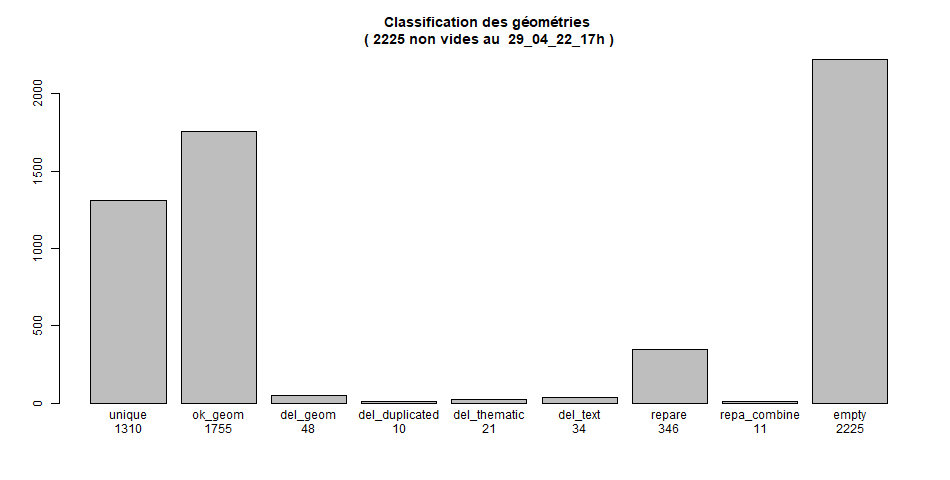
\includegraphics{./figures/bar_classify_Del_29_04_22_17h.png}

}

\caption{Chart Bar des NAS}

\end{figure}

Voici un graphique produit avec \texttt{R} et dot on peut lire le
(court) script

\begin{Shaded}
\begin{Highlighting}[numbers=left,,]
\FunctionTok{plot}\NormalTok{(cars)}
\FunctionTok{plot}\NormalTok{(pressure)}
\end{Highlighting}
\end{Shaded}

\begin{figure}

\begin{minipage}[t]{0.50\linewidth}

{\centering 

\raisebox{-\height}{

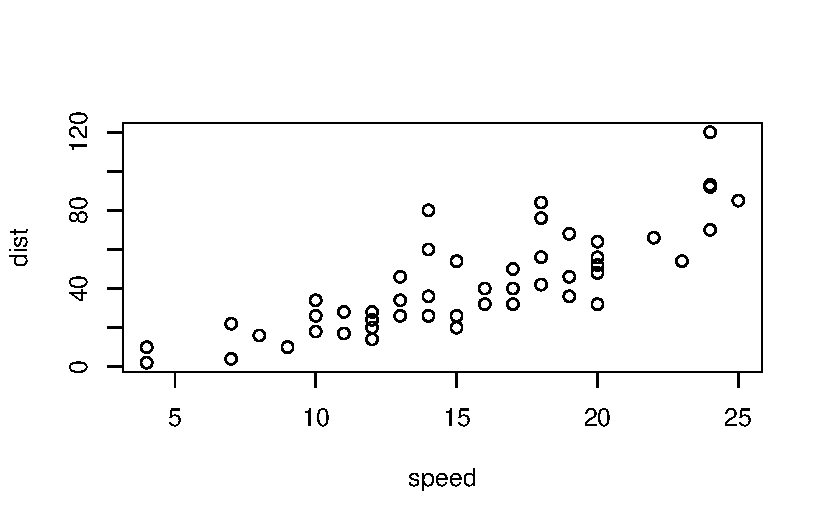
\includegraphics{./resultats_files/figure-pdf/unnamed-chunk-1-1.pdf}

}

\caption{Speed and Stopping Distances of Cars}

}

\end{minipage}%
%
\begin{minipage}[t]{0.50\linewidth}

{\centering 

\raisebox{-\height}{

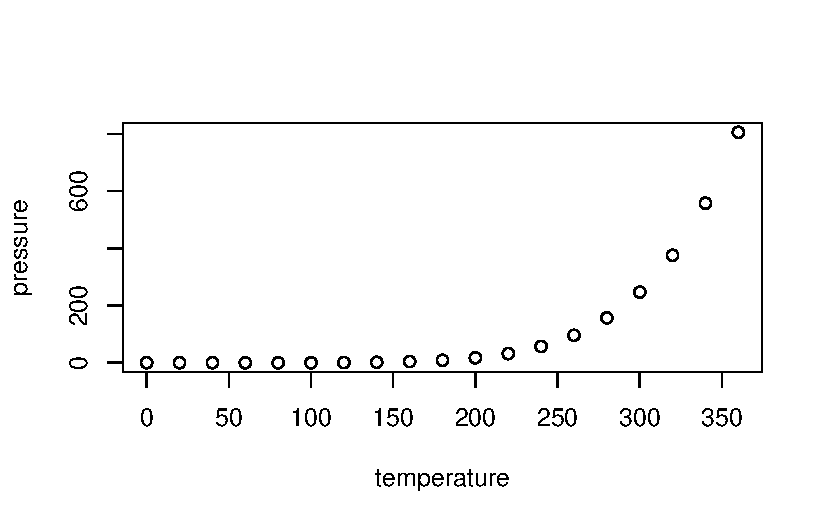
\includegraphics{./resultats_files/figure-pdf/unnamed-chunk-1-2.pdf}

}

\caption{Vapor Pressure of Mercury as a Function of Temperature}

}

\end{minipage}%

\end{figure}

Ceci est un exemple de diagramme écrit en \texttt{mermaid}

\begin{Shaded}
\begin{Highlighting}[numbers=left,,]

\NormalTok{flowchart LR}
\NormalTok{  A[Hard edge] {-}{-}\textgreater{} B(Round edge)}
\NormalTok{  B {-}{-}\textgreater{} C\{Decision\}}
\NormalTok{  C {-}{-}\textgreater{} D[Result one]}
\NormalTok{  C {-}{-}\textgreater{} E[Result two]}
\end{Highlighting}
\end{Shaded}

\begin{figure}[H]

{\centering 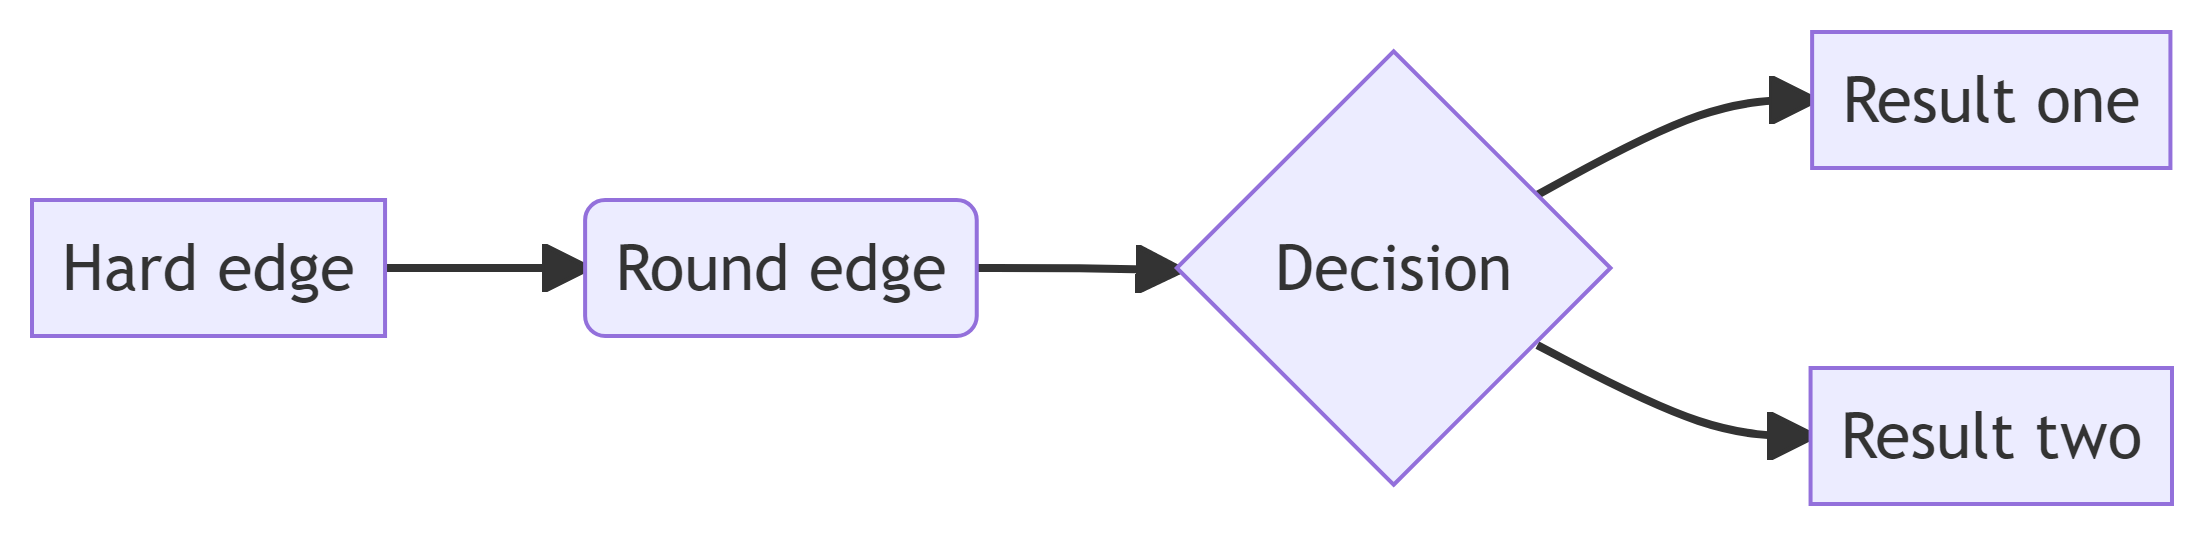
\includegraphics[width=5.74in,height=1.4in]{./resultats_files/figure-latex/mermaid-figure-1.png}

}

\end{figure}

Un autre exemple de diagramme

\begin{figure}[H]

{\centering 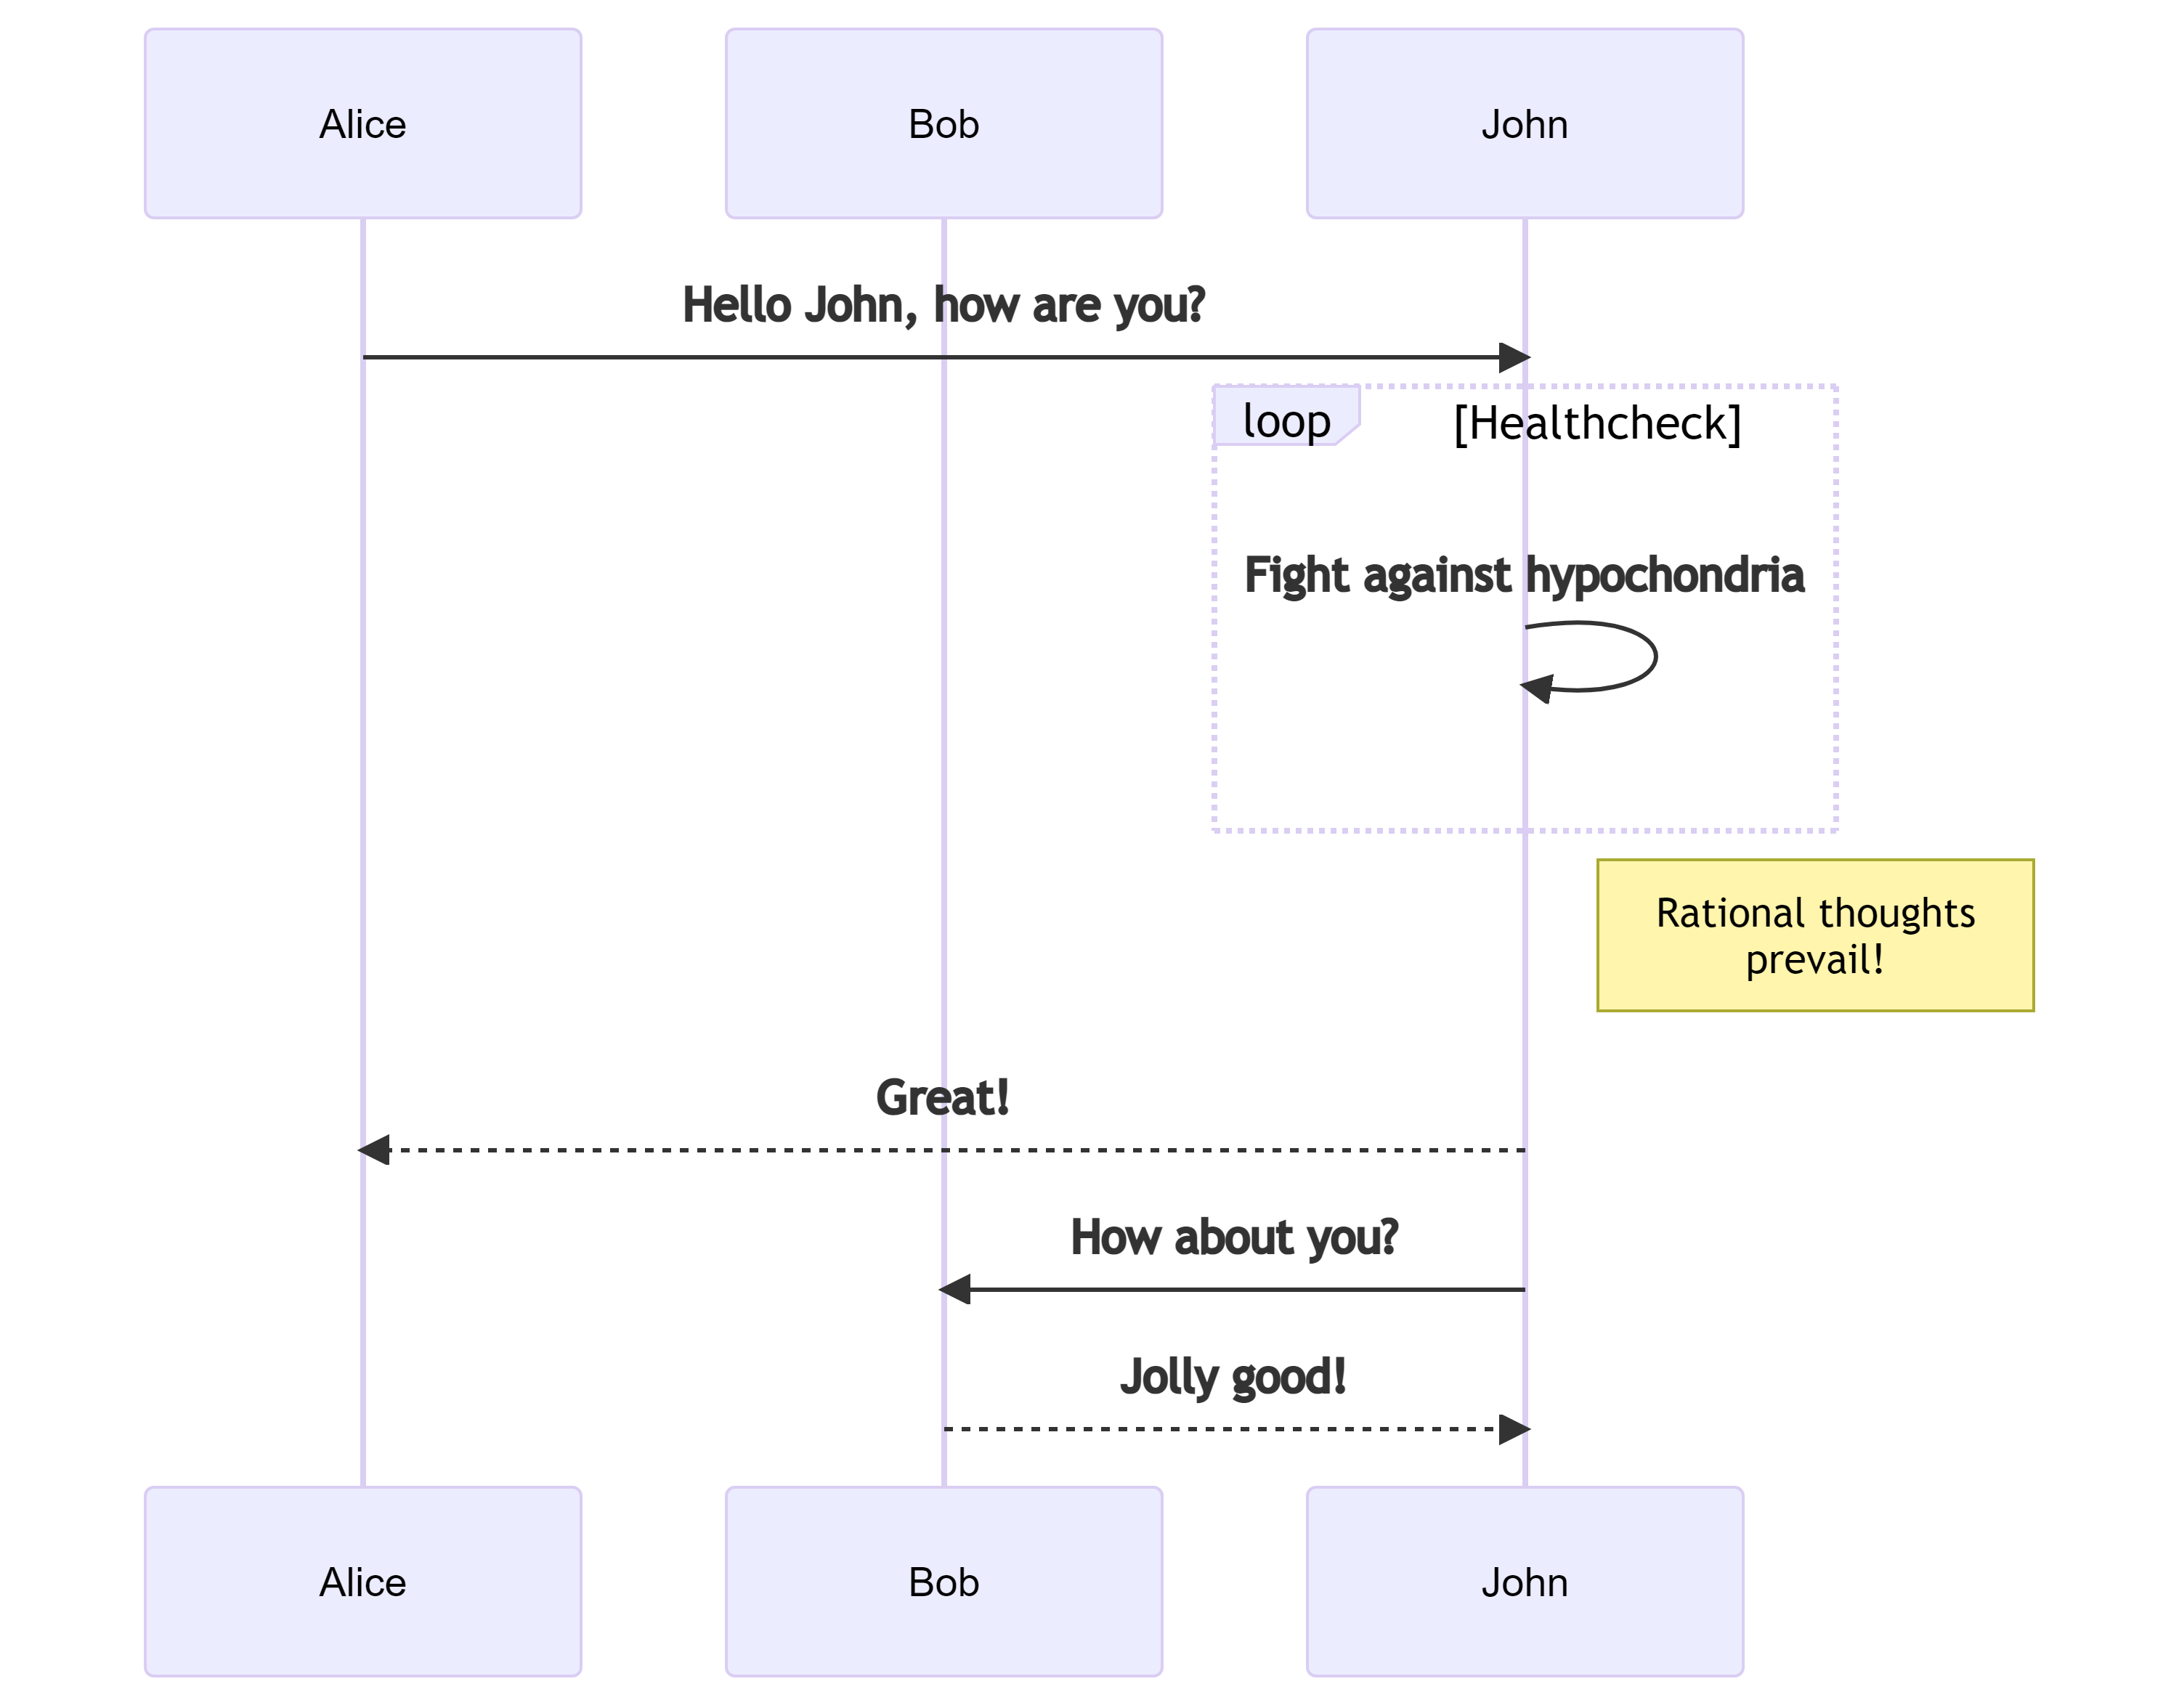
\includegraphics[width=5.33in,height=5.33in]{./resultats_files/figure-latex/mermaid-figure-2.png}

}

\end{figure}

\hypertarget{data}{%
\section{Data}\label{data}}

The penguins data from the
\href{https://allisonhorst.github.io/palmerpenguins}{\textbf{palmerpenguins}}
package contains size measurements for r nrow(penguins) penguins from
three species observed on three islands in the Palmer Archipelago,
Antarctica./ The plot below shows the relationship between flipper and
bill lengths of these penguins.

\begin{Shaded}
\begin{Highlighting}[numbers=left,,]
\FunctionTok{library}\NormalTok{(palmerpenguins)}
\FunctionTok{library}\NormalTok{(ggplot2)}
\FunctionTok{ggplot}\NormalTok{(penguins, }
       \FunctionTok{aes}\NormalTok{(}\AttributeTok{x =}\NormalTok{ flipper\_length\_mm, }\AttributeTok{y =}\NormalTok{ bill\_length\_mm)) }\SpecialCharTok{+}
  \FunctionTok{geom\_point}\NormalTok{(}\FunctionTok{aes}\NormalTok{(}\AttributeTok{color =}\NormalTok{ species, }\AttributeTok{shape =}\NormalTok{ species)) }\SpecialCharTok{+}
  \FunctionTok{scale\_color\_manual}\NormalTok{(}\AttributeTok{values =} \FunctionTok{c}\NormalTok{(}\StringTok{"darkorange"}\NormalTok{,}\StringTok{"purple"}\NormalTok{,}\StringTok{"cyan4"}\NormalTok{)) }\SpecialCharTok{+}
  \FunctionTok{labs}\NormalTok{(}
    \AttributeTok{title =} \StringTok{"Flipper and bill length"}\NormalTok{,}
    \AttributeTok{subtitle =} \StringTok{"Dimensions for penguins at Palmer Station LTER"}\NormalTok{,}
    \AttributeTok{x =} \StringTok{"Flipper length (mm)"}\NormalTok{, }\AttributeTok{y =} \StringTok{"Bill length (mm)"}\NormalTok{,}
    \AttributeTok{color =} \StringTok{"Penguin species"}\NormalTok{, }\AttributeTok{shape =} \StringTok{"Penguin species"}
\NormalTok{  ) }\SpecialCharTok{+}
  \FunctionTok{theme\_minimal}\NormalTok{()}
\end{Highlighting}
\end{Shaded}

\begin{figure}[H]

{\centering 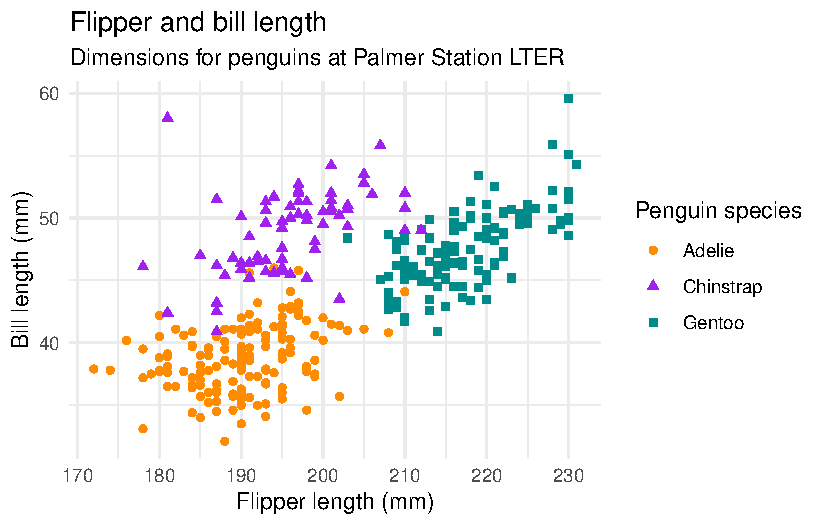
\includegraphics{./resultats_files/figure-pdf/plot-penguins-1.pdf}

}

\end{figure}

\bookmarksetup{startatroot}

\hypertarget{conclusion}{%
\chapter{Conclusion}\label{conclusion}}

Dans quelles conditions peut-on la généraliser ? Quelles réponses ont
été données ? Quelles sont celles qui ne l'ont pas été ? Que faut-il
envisager pour l'avenir ?

\bookmarksetup{startatroot}

\hypertarget{remerciements-uxe9ventuels}{%
\chapter{Remerciements éventuels}\label{remerciements-uxe9ventuels}}

\bookmarksetup{startatroot}

\hypertarget{references}{%
\chapter*{References}\label{references}}
\addcontentsline{toc}{chapter}{References}

\hypertarget{refs}{}
\begin{CSLReferences}{0}{0}
\end{CSLReferences}

\appendix
\addcontentsline{toc}{part}{Appendices}

\hypertarget{sec-more-results}{%
\chapter{More results}\label{sec-more-results}}

Some results that wouldn't fit into the main thesi

Some results that wouldn't fit into the main thesis

\begin{figure}

{\centering 
\includegraphics{./cover.png}

}

\caption{cover}

\end{figure}


\backmatter

\end{document}
